
O setor de jogos digitais está expansão, prevendo-se que ultrapasse os US\$ 200 bilhões em 2023, conforme indicação de \citeonline{quanto_games_vao_movimentar}. No ano de 2022, somente na plataforma Steam, foram lançados 10.644 novos títulos, e em 2023 até seis de Outubro foram lançados 9,103 jogos, conforme evidenciado pela \cref{fig:steam_publishes} existe uma tendência do aumento de lançamentos de jogos na Steam ao decorrer dos anos.


\begin{figure}[!ht]
	\centering
    \caption{número de jogos publicados na Steam.}
	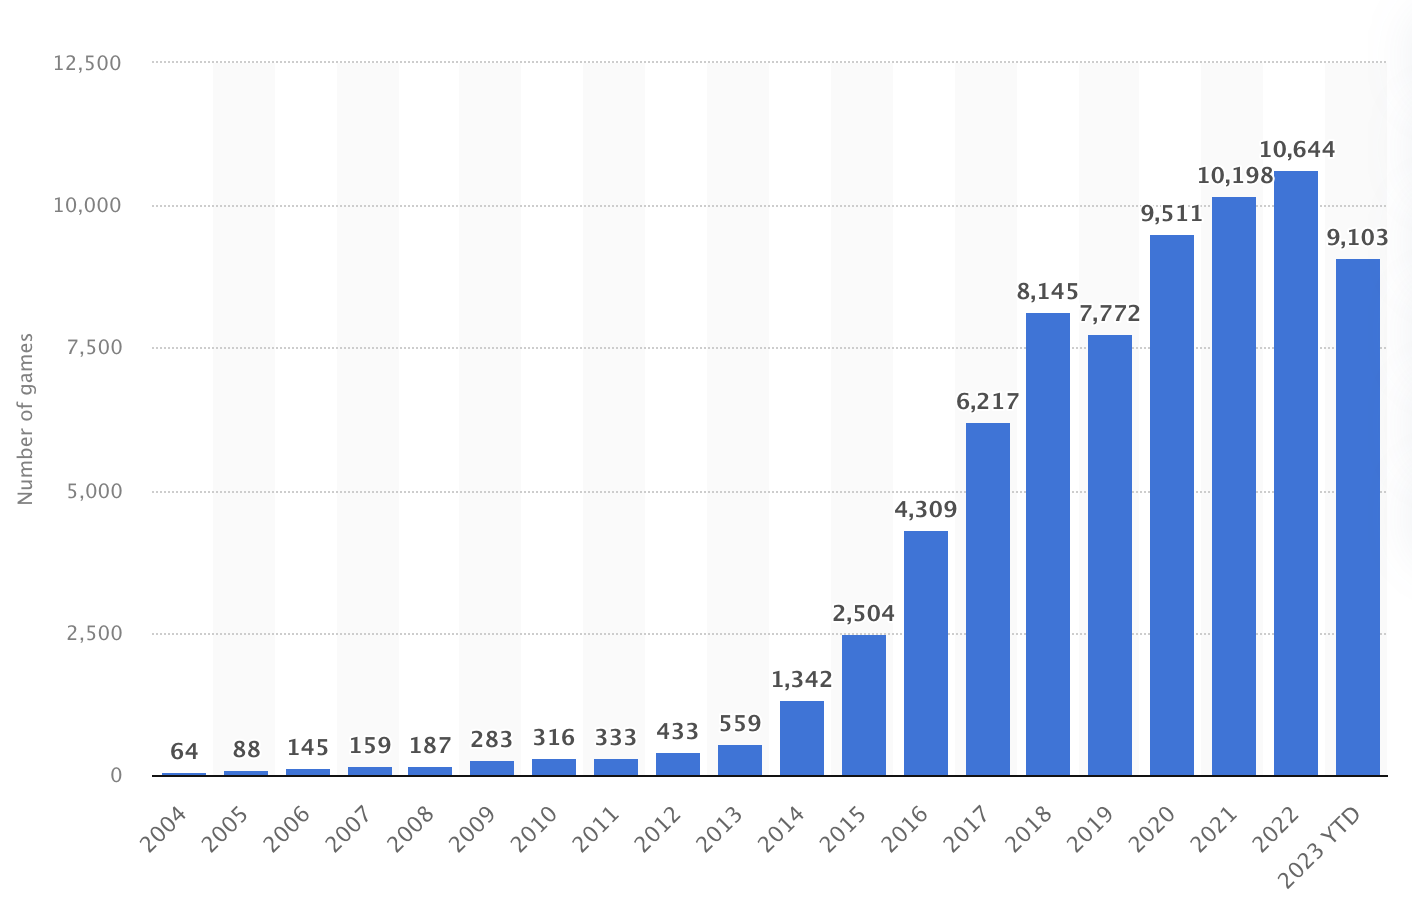
\includegraphics[width=0.6\textwidth]{figures/steam_sales.png}
	\legend{Fonte: \citeonline{numero_de_jogos_publicados_na_steam}}
	\label{fig:steam_publishes}
\end{figure}

Dentro do universo dos jogos, os mapas assumem um papel fundamental, não apenas orientando os jogadores, mas também enriquecendo a experiência ao criar uma sensação de escala e proporcionar uma exploração mais rica \space\cite{video_game_maps, minimap}.

Na elaboração de mapas, emprega-se uma técnica denominada geração procedural, a qual se baseia na criação dinâmica de conteúdo por meio de algoritmos. Essa abordagem surgiu com o propósito de gerar mapas durante a execução de um programa e minimizar as demandas de armazenamento, uma vez que havia restrições nesse aspecto na época. Contudo, mesmo diante da superação dessas limitações nos dias atuais, a geração procedural persiste como uma estratégia aplicada para a produção de conteúdos exclusivos a cada execução do programa \cite{kenny2021procedural, lambda3}.

Na abordagem da geração procedural, várias técnicas são exploradas, conforme discutido por \citeonline{kvrivzmulti}. Dentre essas, destacam-se o \textit{Perlin Noise}, útil na criação de contornos e texturas de aparência natural, os \textit{L-systems}, empregados na geração de vegetação, o \textit{Voronoi}, utilizado para a criação de texturas e a partição de espaços 2D, e os autômatos celulares, aplicados na criação de cavernas em 2D, entre outras abordagens.

Na geração procedural existem desafios, como por exemplo descrito por \citeonline{geracao_procedural_jogos_2d} "Um dos maiores desafios  no desenvolvimento de algoritmos para geração de mapas é  a  dificuldade  de  se  criar  cenários  que  sejam,  ao mesmo  tempo,  atraentes  e diversificados,  permitindo que o jogador possa explorar um novo ambiente a cada sessão de jogo" \space\cite{geracao_procedural_jogos_2d}.




Com o objetivo de gerar mapas com biomas de forma procedural com personalização de IA, decidiu-se utilizar o resultado da segmentação de imagem por rede neural convolucional para o usuário selecionar uma área e assim delimitar o contorno da ilha, adicionando, portanto, uma personalização. Essa aplicação possibilita um desenvolvedor de jogos criar um protótipo de mapa rapidamente ou aprimorar e usar esse recurso no jogo, possibilitando o jogador tirar ou selecionar uma foto e escolher um contorno para gerar um mapa com aquele formato.

Por fim, para contribuição científica tem-se a hipótese de que quanto mais pontos o diagrama de Voronoi tiver maior será a precisão da compatibilidade entre o mapa gerado e o contorno escolhido. Para chegar a essa conclusão, comprometeu-se definir alguns testes com métricas em prol de mensurar a qualidade da geração procedural com o contorno selecionado.

\section{Objetivos}

O objetivo principal deste trabalho é desenvolver uma ferramenta que ofereça uma alternativa para a geração procedural de mapas de ilhas, utilizando o diagrama de Voronoi para a criar biomas. Além disso, pretende-se combinar segmentação com redes neurais convolucionais para permitir a personalização desses mapas. Essa ferramenta terá a capacidade de reconhecer os contornos reconhecidos (classificados no conjunto de dados, logo o resultado terá uma detecção abrangente dentro do escopo de classes obtidas) de uma imagem, e gerar um mapa com um mapa baseado nos limites do contorno escolhido.

Adicionalmente, os seguintes objetivos específicos serão abordados:

\begin{itemize}
	\item Selecionar e analisar conjuntos de dados contendo classes relevantes, como pessoas, carros, entre outros, para treinar um modelo de rede neural convolucional específico para segmentação de imagens.
	\item Utilizar algoritmos para criar diagramas de Voronoi.
	\item Aplicar um algoritmo para reconhecer a imagem com o contorno selecionado e gerar como resultado a imagem do mapa gerado.
	\item Utilizar o resultado da segmentação para selecionar indicar o que é terreno em cima do diagrama de Voronoi.
	\item Gerar os biomas no diagrama de Voronoi.
	\item Criar testes em prol de mensurar a semelhança entre o contorno do mapa gerado com o contorno escolhido.
\end{itemize}